\documentclass[journal]{IEEEtran}
\usepackage{amsmath,amssymb,amsthm,bm}
\usepackage{graphicx,booktabs,array,multirow,cite}
\usepackage{algorithm,algpseudocode}
\usepackage[hidelinks]{hyperref}
\newtheorem{proposition}{Proposition}
\newtheorem{corollary}{Corollary}
\newtheorem{lemma}{Lemma}
\DeclareMathOperator{\conv}{conv}
\DeclareMathOperator*{\argmin}{arg\,min}
\newcommand{\R}{\mathbb R}
\newcommand{\bp}{\bm p}
\newcommand{\bu}{\bm u}
\newcommand{\blambda}{\bm\lambda}
\newcommand{\Pmin}{P^{\min}}
\newcommand{\Pmax}{P^{\max}}
\newcommand{\UC}{\mathrm{UC}}
\newcommand{\SSched}{\mathrm{SS}}
\newcommand{\CHP}{\mathrm{CHP}}
\begin{document}
\title{Parametric Convex Hull Pricing for Strategic Offer Evaluation and Market Power Analysis}
\author{Chen Ling, and~Chenye Wu,~\IEEEmembership{Senior Member,~IEEE}%
\thanks{C. Ling and C. Wu are with the School of Science and Engineering, The Chinese University of Hong Kong (Shenzhen), Shenzhen 518172, Guangdong, China, and also with Shenzhen Loop Area Institute, Shenzhen 518045, Guangdong, China.}}
\maketitle

\begin{abstract}
Convex hull pricing reduces the compensation associated with nonconvex generation costs, while strategic offers can still change prices, dispatch, and producer profits. Evaluating these opportunities over a continuous offer range requires repeated pricing and consistent treatment of physical scheduling and uplift. This paper develops a parametric pricing and strategic offer evaluation framework for network-constrained, multiperiod markets. A common optimal primal solution and complete endpoint dual solutions define reusable affine price selections. Combining these price segments with common optimal unit commitment schedules reduces profit maximization along a specified offer direction to finitely many boundary candidates. Under complete reported lost-opportunity-cost compensation, a profit identity separates price effects from the difference between scheduled and self-scheduled offer exposure. Substitution cost thresholds and a controlled transmission intervention explain how physical competition shapes profitable offers. Measured pricing speedups reach 6.74 and 20.54 on the 30-bus system, and 2.00 on the longer 118-bus workload. The shorter 118-bus workload has not amortized preprocessing. In the principal case, additional profit reaches 7,811.56 dollars while uplift decreases by 578.36 dollars. Transmission relaxation changes both nodal price differences and feasible substitution, and its effect on additional profit differs from its effect on total profit.
\end{abstract}
\begin{IEEEkeywords}
Convex hull pricing, market power, parametric optimization, strategic offers, unit commitment, uplift payment.
\end{IEEEkeywords}

\section{Introduction}
\IEEEPARstart{C}{onvex} hull pricing (CHP) incorporates unit commitment nonconvexities into electricity price formation by pricing the convexified system cost. Its settlement interpretation connects energy prices with the compensation needed to support executable generation schedules~\cite{gribik2007,hua2017}. This connection raises an economic question for market monitoring: when a generator changes its offer, how does its influence on CHP translate into additional actual profit? Answering this question requires prices, physical dispatch, and uplift to be evaluated together over the generator's admissible strategy range.

Two strands of CHP market-power research motivate this question. Sun \emph{et al.}~\cite{sun2020market,sun2021strategic} characterized profitable offer manipulation and related potential market power to the cost of removing a generator. Wu and Sun~\cite{wu2021potential} further examined fixed- and variable-cost offers. Sun and Wu~\cite{sun2021temporal} studied how offers propagate through multiperiod CHP prices and developed temporal vulnerability measures from price sensitivities. These studies establish complementary economic objects: the ability to influence prices and the ability to profit from exercising that influence. Their connection becomes more involved when generators can start and stop within the horizon, ramp between hours, and compete through a constrained transmission network.

The computational foundations for studying these interactions are now available. Convex primal and extended unit commitment formulations provide representations of the power--cost sets required for CHP~\cite{hua2017,pan2018,yu2019,networkflow}. Decomposition methods also obtain CHP from unit-level subproblems~\cite{andrianesis2022dw}. Network-flow models organize feasible operating intervals, while perspective constraints attach continuous output and operating cost to the same interval weights. Parametric descriptions offer a further opportunity to reuse optimization structure. For example, the demand-to-price interpretation in~\cite{jiang2026minkowski} illustrates how a mapping can expose price formation across changing market inputs. Strategic offer analysis instead changes objective coefficients and must also retain the integer physical schedules used for settlement.

A sequence of isolated offer evaluations obscures the boundaries at which price responses or executable schedules change. Local price derivatives alone also omit the economic consequences of dispatch replacement and the difference between reported and actual costs. A generator may earn more while receiving less uplift; two equally costly physical schedules can produce different actual profits at the same selected CHP. A useful evaluation method must preserve these distinctions while making a continuous offer range computationally accessible.

This paper develops such a framework for a specified affine offer direction. The first contribution is a reusable parametric CHP representation coupled with finite strategic-profit evaluation. Common primal optima and complete optimal endpoint duals certify affine price selections without requiring a particular simplex basis. Their intersection with common optimal physical schedules yields intervals on which actual profit is convex, reducing the declared strategy evaluation to boundary candidates. The second contribution is an economic characterization of profitable market power under complete reported lost-opportunity-cost compensation. The characterization connects price responses, scheduled versus self-scheduled offer exposure, physical substitution thresholds, and network constraints. It supports controlled interpretations of how operating costs and transmission capacity change the opportunity to earn additional profit.

The numerical studies retain both preprocessing and query costs, including independent short and longer 118-bus workloads. The principal 30-bus case then connects continuous prices to complete producer settlement, a predictable substitution threshold, and a single-line transmission intervention. The results show why price influence, total producer profit, and additional profit relative to truthful bidding answer different market questions.

\section{Market Model and Strategic Offers}\label{sec:model}
\subsection{Physical Scheduling and Offer Direction}
Let $\mathcal G$, $\mathcal B$, and $\mathcal L$ denote generators, buses, and lines, and let $t\in\mathcal T=\{1,\ldots,T\}$. Generator $g$ is connected to bus $n(g)$. Its physical schedule is $s_g=(\bp_g,\bu_g)\in\mathcal S_g$, where $u_{g,t}\in\{0,1\}$ and $p_{g,t}$ is output. The set $\mathcal S_g$ includes minimum up/down times, inherited operating conditions, and
\begin{subequations}\label{eq:physical}
\begin{align}
 \Pmin_g u_{g,t}&\le p_{g,t}\le\Pmax_g u_{g,t},\\
 p_{g,t}-p_{g,t-1}&\le R_g^\uparrow\quad (u_{g,t-1}=u_{g,t}=1),\\
 p_{g,t-1}-p_{g,t}&\le R_g^\downarrow\quad (u_{g,t-1}=u_{g,t}=1),\\
 p_{g,t}&\le S_g^\uparrow\quad (u_{g,t-1}=0,\ u_{g,t}=1),\\
 p_{g,t-1}&\le S_g^\downarrow\quad (u_{g,t-1}=1,\ u_{g,t}=0).
\end{align}
\end{subequations}
The initial status, power, and residual minimum up/down times are part of the fixed market instance. Model identity is retained across physical scheduling and pricing because CHP can depend on the underlying primal formulation~\cite{zhao2023dependence}. No artificial shutdown is imposed at the horizon end.

For one-hour intervals, actual operating cost is
\begin{align}
 C_g(s_g)={}&C_g^{\mathrm{SU}}n_g^{\mathrm{SU}}+C_g^{\mathrm{SD}}n_g^{\mathrm{SD}}
 +C_g^{\mathrm{NL}}\sum_tu_{g,t}\notag\\[-2pt]
 &+\sum_t\phi_g(p_{g,t}-\Pmin_g u_{g,t}),\label{eq:cost}
\end{align}
where $\phi_g$ is convex piecewise linear and $C_g^{\mathrm{NL}}$ covers operation at minimum output. Startup and shutdown charges apply to actual in-horizon transitions. For a target generator $g$, define the quantity exposed to the offer increase by
\begin{equation}
 Q_g(s_g)=\sum_t w_t(p_{g,t}-\Pmin_g u_{g,t}),\qquad w_t\ge0.\label{eq:exposure}
\end{equation}
The reported cost is $\widehat C_g(s_g;\delta)=C_g(s_g)+\delta Q_g(s_g)$, with $\delta\in[0,\bar\delta]$. All other generators report their actual costs. The principal strategy uses $w_t=1$ throughout the day; an hour-specific direction uses one nonzero weight. The scalar $\delta$ is an absolute incremental-cost adder in dollars per megawatt-hour.

Let $H_{\ell n}$ be the PTDF and $F_\ell$ the line limit. With demand $D_{n,t}$, the system-feasible set $\mathcal F^{\UC}$ imposes $s_i\in\mathcal S_i$ and
\begin{align}
 \sum_i p_{i,t}&=\sum_n D_{n,t},\label{eq:balance}\\
 f_{\ell,t}&=\sum_iH_{\ell,n(i)}p_{i,t}-\sum_nH_{\ell n}D_{n,t},\label{eq:network}\\
 -F_\ell&\le f_{\ell,t}\le F_\ell.\notag
\end{align}
The independent system operator selects an executable schedule $s^{\UC}(\delta)$ minimizing the total reported cost over $\mathcal F^{\UC}$. Denote its optimal value by $v^{\UC}(\delta)$.

\subsection{CHP Through a Direct-Power Extended Formulation}
CHP convexifies each generator's joint power--cost epigraph while retaining the system balance and network constraints. The extended representation used here follows the operating-interval and network-flow construction in~\cite{pan2018,networkflow}. An alternating time-expanded directed acyclic graph connects feasible ON and OFF intervals into complete commitment paths. Minimum up/down times and initial conditions determine allowable arcs. A unit source-to-sink flow $z_{g,e}$ represents a convex combination of these paths.

For an ON arc $e=[a,b]$, introduce scaled power $p_{g,e,t}$ directly. Its perspective dispatch constraints include
\begin{subequations}\label{eq:interval}
\begin{align}
 \Pmin_g z_{g,e}&\le p_{g,e,t}\le\Pmax_g z_{g,e},&&a\le t\le b,\\
 p_{g,e,t}-p_{g,e,t-1}&\le R_g^\uparrow z_{g,e},&&a<t\le b,\\
 p_{g,e,t-1}-p_{g,e,t}&\le R_g^\downarrow z_{g,e},&&a<t\le b.
\end{align}
\end{subequations}
A new startup gives $p_{g,e,a}\le S_g^\uparrow z_{g,e}$; an actual following shutdown gives $p_{g,e,b}\le S_g^\downarrow z_{g,e}$. Inherited online arcs instead use the preceding power and normal ramp limits. Terminal ON arcs incur no artificial shutdown. If $\phi_g(q)=\max_k\{a_{gk}q+b_{gk}\}$, the interval cost variables satisfy
\begin{equation}
 \xi_{g,e,t}\ge a_{gk}(p_{g,e,t}-\Pmin_g z_{g,e})+b_{gk}z_{g,e},\quad\forall k.\label{eq:perspective}
\end{equation}
Output, commitment, and cost aggregate under the same arc weights. Summing $p_{g,e,t}$ and $z_{g,e}$ over ON arcs covering $t$ recovers unit output and commitment; fixed interval costs and $\xi$ recover cost. Thus ramping is expressed through consecutive physical outputs, without differential-power coordinates. This formulation supplies the pricing feasible set; the contribution studied below is its parametric and strategic use.

For fixed physical parameters and an affine offer direction, the pricing problem has the form
\begin{align}
 v^{\CHP}(\delta)&=\min_{x\in\mathcal P}(c^0+\delta d)^\top x,\label{eq:paramlp}\\
 \mathcal P&=\{x:Ax=b,\ Gx\le h,\ \ell\le x\le u\}.\notag
\end{align}
Here $x$ collects arc-flow, direct-power, and cost variables. The feasible set is independent of $\delta$; $d$ represents~\eqref{eq:exposure}. The convexified pricing output $\bp^{\CHP}$ can be fractional in commitment and differs from the executable $\bp^{\UC}$.

Let $\lambda_t^E$ be the multiplier on system balance, with nonnegative multipliers $\mu_{\ell,t}^{+}$ and $\mu_{\ell,t}^{-}$ on the upper and lower line limits. Nodal CHP is
\begin{equation}
 \lambda_{n,t}^{\CHP}=\lambda_t^E+\lambda_{n,t}^C,\qquad
 \lambda_{n,t}^C=-\sum_\ell H_{\ell n}(\mu_{\ell,t}^+-\mu_{\ell,t}^-).\label{eq:lmp}
\end{equation}
The system energy component is the balance multiplier of the constrained problem. Both components depend on the PTDF reference; nodal prices and settlement are invariant under a consistent reference change.

\subsection{Self-Scheduling, Uplift, and Actual Profit}
Given the announced nodal price vector $\blambda_g$, a generator's best reported self-scheduling profit is
\begin{equation}
 \widehat\Pi_g^{\SSched}(\blambda_g,\delta)=\max_{s_g\in\mathcal S_g}
 \{\blambda_g^\top\bp_g-\widehat C_g(s_g;\delta)\}.\label{eq:ss}
\end{equation}
Its optimizer $s_g^{\SSched}$ satisfies unit operating constraints; the collection of unit best responses need not balance system demand or satisfy network limits. This is the third dispatch object, distinct from physical clearing and convexified pricing output.

Actual energy revenue, uplift payment, and actual profit are
\begin{align}
 R_g(\delta)&=\blambda_g^{\CHP}(\delta)^\top\bp_g^{\UC}(\delta),\label{eq:revenue}\\
 U_g(\delta)&=\widehat\Pi_g^{\SSched}-[R_g(\delta)-\widehat C_g(s_g^{\UC};\delta)],\label{eq:uplift}\\
 \Pi_g(\delta)&=R_g(\delta)+U_g(\delta)-C_g(s_g^{\UC}(\delta)).\label{eq:profit}
\end{align}
Throughout this paper, uplift means the complete reported lost-opportunity-cost payment in~\eqref{eq:uplift}. Since $s_g^{\UC}$ is feasible for~\eqref{eq:ss}, $U_g\ge0$. Reported cost determines compensation, whereas actual operating cost determines actual profit.

For fixed other offers, the additional-profit objective is
\begin{equation}
 \mathcal M_g=\max_{\delta\in[0,\bar\delta]}\Delta\Pi_g(\delta),\qquad
 \Delta\Pi_g(\delta)=\Pi_g(\delta)-\Pi_g(0).\label{eq:marketpower}
\end{equation}
This definition binds market power to the specified direction, offer range, price selection, and physical execution rule. We construct one legal price selection by complete-dual interpolation. Each open physical region executes its archived common optimum; at a shared boundary we evaluate both adjacent plans and select the higher-profit candidate. The rule makes the economic object reproducible and exposes the value of physical tie selection.

\section{Parametric Pricing and Finite Offer Evaluation}\label{sec:method}
\subsection{Common Primal Solutions and Complete Dual Interpolation}
The value of~\eqref{eq:paramlp} is concave and piecewise affine because it is the pointwise minimum of affine functions of $\delta$. A price selection requires the complete optimal dual information, including multipliers on variable bounds. Denote a complete dual vector by $y$, its feasible set at offer $\delta$ by $\mathcal D(\delta)$, and its dual objective by $L(y)$. Dual feasibility includes stationarity with $c^0+\delta d$ and the signs on inequality and bound multipliers. The right-hand sides are fixed, so $L$ is linear and does not depend explicitly on $\delta$.

\begin{proposition}[Affine selected prices]\label{prop:dual}
Suppose a feasible $\bar x$ is optimal at $a<b$, and complete dual optima $y^a\in\mathcal D(a)$ and $y^b\in\mathcal D(b)$ attain its endpoint costs. For $\delta=(1-\theta)a+\theta b$, $0\le\theta\le1$, the vector $y(\delta)=(1-\theta)y^a+\theta y^b$ is dual optimal. Its nodal-price projection is affine on $[a,b]$.
\end{proposition}
\begin{proof}
Interpolating stationarity gives the objective $c^0+\delta d$. All multiplier sign conditions are preserved. Moreover,
\begin{align*}
 L(y(\delta))&=(1-\theta)L(y^a)+\theta L(y^b)\\
 &=(c^0+\delta d)^\top\bar x.
\end{align*}
Primal and dual feasibility with equal objectives establish optimality. Nodal prices are a linear projection of the balance and line multipliers in~\eqref{eq:lmp}.
\end{proof}

The proposition retains all relevant multipliers and does not depend on a nondegenerate basis. Shared endpoint duals also define a continuous price selection across adjacent intervals. Different legal selections may exist; the stored selection determines the profit evaluation.

\subsection{Adaptive Construction and Repeated Queries}
At solved offers $\delta_i$, store primal solutions $x^i$, complete duals, and the affine feasible-cost lines
\begin{equation}
 \ell_i(\delta)=(c^0)^\top x^i+\delta d^\top x^i.\label{eq:primal-line}
\end{equation}
These lines upper-bound $v^{\CHP}$. On a bracket $[a,b]$, the chord between endpoint optimal values lower-bounds the concave value function. The gap between the lower chord and the minimum of the two endpoint feasible-cost lines identifies an interior point where additional optimization is most informative. If a saved feasible primal is optimal at both endpoints, Proposition~\ref{prop:dual} opens the whole bracket for price queries. Otherwise the bracket is refined.

The implementation updates only objective coefficients in a persistent pricing model. A bracket is accepted after checking primal feasibility, complete dual feasibility, strong duality, and the common-primal endpoint gaps. The numerical thresholds are recorded separately from the exact statements above. Completed brackets can be merged for value representation when one common primal covers the union. Collinear nodal-price segments can be compressed separately while preserving the selected price path. Consequently, the number of price segments need not equal the number of value segments.

An online query locates its stored segment and evaluates affine value and price formulas. With $K$ segments, location takes $O(\log K)$ comparisons, followed by the arithmetic needed to return the requested prices. Offline construction remains an optimization task. The cumulative cost comparison therefore includes construction, postprocessing, loading, and measured lookup, rather than treating preprocessing as free.

\subsection{Common Physical Regions and Finite Candidates}
For a complete physical system schedule $s$, define its cost line
\begin{equation}
 \ell_s^{\UC}(\delta)=C_{\mathrm{sys}}(s)+\delta Q_g(s_g),\label{eq:uc-line}
\end{equation}
where $C_{\mathrm{sys}}$ uses actual costs. Since the physical feasible set is fixed, $v^{\UC}$ is also the minimum of affine lines and hence concave, despite the integer commitment decisions. Global mixed-integer lower bounds supply the corresponding endpoint certificate.

\begin{lemma}[Common physical schedule]\label{lem:uc}
If one system-feasible schedule attains $v^{\UC}(a)$ and $v^{\UC}(b)$, it is optimal throughout $[a,b]$.
\end{lemma}
\begin{proof}
The feasible schedule line upper-bounds $v^{\UC}$. Concavity lower-bounds $v^{\UC}$ by its endpoint chord. Endpoint equality makes this chord identical to the schedule line.
\end{proof}

Intersect common physical regions with affine selected-price segments. On each resulting joint interval $I$, fix a common physical optimum $s^{\UC,I}$ and use $\blambda_g(\delta)=\alpha_g+\delta\beta_g$. The following result gives the candidate reduction.

\begin{proposition}[Finite profit evaluation]\label{prop:finite}
Assume a fixed unit feasible set, fixed actual cost, complete reported uplift, an affine selected price on $I=[a,b]$, and a common physical optimum executed on $I$. Then $\Pi_g^I(\delta)$ is convex and
\begin{equation}
 \max_{\delta\in[a,b]}\Pi_g^I(\delta)=\max\{\Pi_g^I(a),\Pi_g^I(b)\}.\label{eq:endpoint}
\end{equation}
Thus a finite joint partition permits evaluation by its endpoint/physical-plan candidates, with the declared boundary execution rule applied explicitly.
\end{proposition}
\begin{proof}
Substitution of~\eqref{eq:uplift} into~\eqref{eq:profit} yields
\begin{equation}
 \Pi_g^I(\delta)=\max_{s_g\in\mathcal S_g}\{a_g(s_g)+\delta b_g(s_g)\}
 +\delta Q_g(s_g^{\UC,I}),\label{eq:convex-profit}
\end{equation}
where $a_g(s_g)=\alpha_g^\top\bp_g-C_g(s_g)$ and $b_g(s_g)=\beta_g^\top\bp_g-Q_g(s_g)$.
Each fixed self-schedule contributes an affine function of $\delta$. Their supremum is convex, and the final term is affine. A convex function on a compact interval does not exceed the larger endpoint value. At a physical boundary, each adjacent plan supplies its own endpoint value under the stated execution rule.
\end{proof}

This result concerns profit rather than the price-response norm alone. It requires physical-region information, but does not require enumerating every self-scheduling region to identify endpoint candidates. Complete profit and uplift curves can subsequently be reconstructed by certifying common optimal self-schedules where needed.

\begin{algorithm}[t]
\caption{Parametric CHP and Strategic Offer Evaluation}\label{alg:workflow}
\begin{algorithmic}[1]
\Require Fixed market instance, direction $Q_g$, domain $[0,\bar\delta]$
\State Solve endpoint CHP problems; retain complete witnesses
\While{an uncertified pricing bracket remains within budget}
\State Check common primal and complete endpoint duals
\State Accept by Proposition~\ref{prop:dual}, or refine the value-gap bracket
\EndWhile
\If{accepted brackets do not cover $[0,\bar\delta]$}
\State \Return certified partial mapping and unresolved brackets
\EndIf
\State Build common physical regions using global UC bounds
\State Require complete physical-region coverage before global profit evaluation
\State Intersect the physical and selected-price partitions
\For{each joint-interval endpoint/physical-plan pair}
\State Solve unit self-scheduling; calculate $R_g,U_g,C_g,\Pi_g$
\EndFor
\State Apply boundary rule and maximize $\Delta\Pi_g$
\end{algorithmic}
\end{algorithm}

\section{Profit Formation and Physical Substitution}\label{sec:mechanism}
\subsection{Profit Identity and Local Channels}
The algebra used in Proposition~\ref{prop:finite} also gives an economic characterization applicable to any feasible physical execution:
\begin{equation}
 \boxed{\Pi_g(\delta)=\widehat\Pi_g^{\SSched}(\blambda_g(\delta),\delta)
 +\delta Q_g(s_g^{\UC}(\delta)).}\label{eq:identity}
\end{equation}
The first term is the highest reported operating profit at the announced prices. The second restores the gap between reported and actual costs on the instructed schedule. At truthful bidding, actual profit equals the best self-scheduling profit. At positive adders, physical selection enters through the offer-exposed quantity.

For two optimal physical schedules $A$ and $B$ at the same offer and selected price,~\eqref{eq:identity} implies
\begin{equation}
 \Pi_g^A-\Pi_g^B=\delta\,[Q_g(s_g^A)-Q_g(s_g^B)].\label{eq:tie-profit}
\end{equation}
Thus equality of the reported system objective and CHP does not imply equality of actual producer profit. The difference is exactly priced by the reported--actual cost discrepancy.

Within a differentiable joint region, an optimal self-schedule gives the envelope relation
\begin{align}
 \frac{d\Pi_g}{d\delta}
 &=\underbrace{(\bp_g^{\SSched})^\top\frac{d\blambda_g^{\CHP}}{d\delta}}_{\text{price effect}}
 +\underbrace{Q_g^{\UC}-Q_g^{\SSched}}_{\text{offer-exposure effect}}\label{eq:derivative}\\
 &=(\bp_g^{\SSched})^\top\frac{d\blambda^E}{d\delta}
 +(\bp_g^{\SSched})^\top\frac{d\blambda_g^C}{d\delta}
 +Q_g^{\UC}-Q_g^{\SSched}.\notag
\end{align}
At self-scheduling switches, the relation applies on the corresponding differentiable sides; integration uses these pieces. A physical switch at a continuous selected price adds the jump $\delta(Q_g^{\UC,+}-Q_g^{\UC,-})$. If a chosen price rule jumps, its contribution must instead be evaluated from the change in the self-scheduling value in~\eqref{eq:identity}. The shared-endpoint rule studied here has continuous prices.

Equation~\eqref{eq:derivative} weights prices by the best self-schedule, whereas energy revenue in~\eqref{eq:revenue} uses actual cleared output. This explains why a positive price-related profit effect and the change in energy revenue have different magnitudes. It also connects temporal price vulnerability to a settlement-based profit measure without equating the two.

\subsection{Substitution Costs and Critical Offers}
Consider two complete physical schedules with actual system costs $C_A,C_B$ and target exposures $Q_A>Q_B$. Their reported cost lines meet at
\begin{equation}
 \delta^*=\frac{C_B-C_A}{Q_A-Q_B}.\label{eq:threshold}
\end{equation}
The numerator measures the additional actual system cost of the alternative; the denominator measures the offer-exposed generation it replaces. A more expensive substitute can sustain a larger offer increase before displacing the current schedule. Interpreting~\eqref{eq:threshold} as an actual clearing threshold requires that no third schedule dominate the two candidates near the crossing. Global UC bounds provide this check.

If a specified cost perturbation changes schedule $j$ by $\epsilon H_j$, the candidate threshold becomes
\begin{equation}
 \delta^*(\epsilon)=\delta^*(0)+\epsilon\frac{H_B-H_A}{Q_A-Q_B}.\label{eq:threshold-shift}
\end{equation}
For an online-cost perturbation, $H_j$ is the substitute's online duration. Equal startup counts instead predict no threshold movement under a startup-cost perturbation. These directions distinguish additional online operation from the cost of initiating that operation.

\subsection{Transmission Prices and Feasible Competition}
Network constraints can affect both terms involved in strategic opportunity. They shape the optimal dual prices in~\eqref{eq:lmp} and restrict the alternative schedules available in~\eqref{eq:uc-line}. Energy/congestion accounting identifies price components under a fixed reference. A controlled change to a line limit additionally reveals changes in feasible competition. These two analyses are used together.

For settlement consistency, define
\begin{equation}
 \Delta^{\mathrm{TX}}=\sum_{\ell,t}
 [\mu_{\ell,t}^+(F_\ell-f_{\ell,t}^{\UC})
 +\mu_{\ell,t}^-(F_\ell+f_{\ell,t}^{\UC})].\label{eq:tx}
\end{equation}
To see the settlement relation, let $D^{\lambda}=\sum_{n,t}\lambda_{n,t}^{\CHP}D_{n,t}$. Strong duality and unit self-scheduling give
\begin{equation}
 v^{\CHP}=D^{\lambda}-\sum_{\ell,t}(\mu_{\ell,t}^++\mu_{\ell,t}^-)F_\ell-\sum_i\widehat\Pi_i^{\SSched}.\label{eq:dual-bridge}
\end{equation}
Equation~\eqref{eq:lmp} and physical balance also give $\sum_iR_i-D^{\lambda}=-\sum_{\ell,t}(\mu_{\ell,t}^+-\mu_{\ell,t}^-)f_{\ell,t}^{\UC}$. Substitution into~\eqref{eq:uplift} yields
\begin{equation}
 \sum_i U_i+\Delta^{\mathrm{TX}}=v^{\UC}(\delta)-v^{\CHP}(\delta).\label{eq:network-settlement}
\end{equation}
The values on the right use reported costs. The nonnegative transmission adjustment evaluates pricing multipliers against physical scheduled flows; it is distinct from a nodal congestion-price component or an individual generator's uplift. In particular, a binding physical line need not have a nonzero CHP multiplier.

\section{Numerical Results}\label{sec:results}
The studies use modified IEEE 30- and 118-bus systems with a 24-hour horizon, three incremental cost segments, and PTDF transmission constraints. The systems have six and 54 generators, respectively. All units are initially offline at zero output with minimum down times satisfied. Every optimization and settlement uses these same inherited conditions. The reference incremental slopes for the principal G1 case and the 118-bus G11 case are 41.982 and 36.33 USD/MWh. The 0--50\% normalized ranges therefore correspond to absolute adders $[0,20.991]$ and $[0,18.165]$ USD/MWh; percentages describe the offer parameter.

The archived timing workloads use COPT 8.0.6 and Python 3.13.5 on the same workstation. Persistent reoptimization includes setup, objective updates, optimization, and price extraction. Parametric totals include construction, postprocessing, loading, and lookup. Queries are fixed shuffled sequences. Physical UC and unit self-scheduling are evaluated separately for settlement; their cost is not included in pricing speedup ratios. Pricing intervals use complete-dual checks and a $10^{-6}$-dollar common-primal acceptance tolerance. Physical regions use global UC bounds with a $10^{-5}$-dollar cost tolerance. These are objective-gap acceptance tolerances, not bounds on dispatch or profit error. The archived checks and source fingerprints are distributed with the results. All reported profits use actual costs after full reported uplift.

\subsection{Computational Performance of Parametric CHP}
\begin{figure*}[t]
\centering
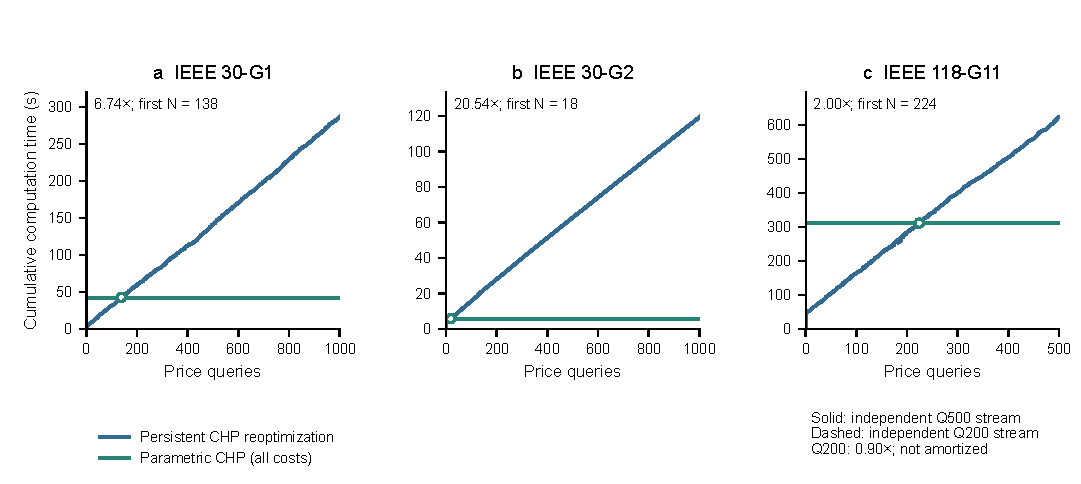
\includegraphics[width=\textwidth]{../paper_results/revision_20261020/figures/fig1_cumulative_pricing_time.pdf}
\caption{Measured cumulative CHP pricing time. The two 30-bus streams contain 1,000 queries each. The 118-bus panel distinguishes independent 500- and 200-query workloads. Parametric totals include construction, postprocessing, loading, and measured lookup. Markers identify first observed amortized query counts; the streams are not concatenated.}
\label{fig:timing}
\end{figure*}
\begin{table}[t]
\centering\caption{Price Mapping and Measured Query Performance}\label{tab:performance}
\setlength{\tabcolsep}{3.4pt}
\begin{tabular}{@{}lrrrrr@{}}\toprule
Instance & Price & Queries & Direct & Param. & Ratio\\
 & segments & & (s) & (s) & \\\midrule
30-G1 &83&1000&286.46&42.52&6.74\\
30-G2 &8&1000&119.28&5.81&20.54\\
118-G11 &103&500&623.41&311.60&2.00\\
118-G11 &103&200&279.35&311.60&0.90\\\bottomrule
\end{tabular}
\vspace{2pt}\parbox{\columnwidth}{\footnotesize Ratio is direct/parametric cumulative time. The 118-bus rows are independent workloads on the same archived mapping. G1 has 17 common physical regions, 99 joint intervals, and 116 endpoint/physical-plan candidates at 100 distinct offers.}
\end{table}
Figure~\ref{fig:timing} and Table~\ref{tab:performance} evaluate the investment in reusable price information. For 30-G1, 1,000 direct queries require 286.46~s, compared with 42.52~s for the complete parametric workflow. The first amortized query is 138. The simpler 30-G2 direction produces eight selected-price segments and reaches amortization at query 18, with a cumulative ratio of 20.54 at 1,000 queries. These differences show that the offer direction and its induced partition matter in addition to system dimensions.

The 118-bus 500-query workload takes 623.41~s by persistent reoptimization and 311.60~s parametrically, reaching first measured amortization at query 224. Its independent 200-query comparison takes 279.35~s directly and 311.60~s parametrically. The short workload illustrates the initial mapping investment; the longer workload demonstrates its reuse. Neither its first 200 observations nor its cumulative sequence substitutes for the independent shorter experiment.

The representation also provides structure for strategy evaluation. G1's 154 saved pricing points support 83 compressed selected-price segments. Seventeen common physical regions yield 99 joint intervals, requiring 116 endpoint/physical-plan evaluations at 100 different offers. Proposition~\ref{prop:finite} converts these into an assessment of the complete declared offer range. The map therefore supplies both repeated pricing and the interval structure needed for economic evaluation.

\subsection{Impact of Strategic Offers on CHP Prices}
\begin{figure*}[t]
\centering
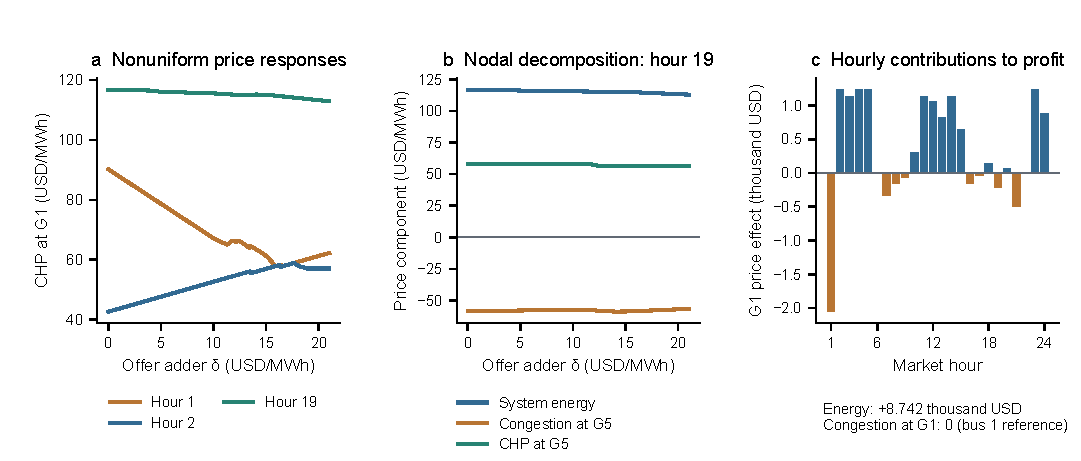
\includegraphics[width=\textwidth]{../paper_results/figures/fig2_energy_congestion_prices.pdf}
\caption{Strategic-offer price responses. (a) G1-node CHP in hours 1, 2, and 19. (b) System energy, congestion, and total CHP at the G5 node in hour 19. (c) Signed hourly contributions to G1's price-related profit effect along the path to the best offer. The PTDF reference is bus 1, where G1 is located. Hour 2 is one of the tied largest positive contribution hours; hour 19 is the baseline demand peak.}
\label{fig:prices}
\end{figure*}
Figure~\ref{fig:prices}(a) shows that increasing a common all-day offer does not raise every hourly CHP. Hour 1 falls markedly, while other hours contribute positively to the target's profit. Integrating the price effect in~\eqref{eq:derivative} gives $+8{,}741.60$ dollars. Positive hourly contributions total $12{,}245.08$, offset by $-3{,}503.47$ from negative hours. Hours 2, 4, 5, and 23 each contribute approximately $1{,}232.38$, whereas hour 1 contributes $-2{,}053.58$. The peak-demand hour contributes approximately $-210.51$. Temporal propagation and the unit's best response jointly determine the economic importance of each price movement.

Bus 1 is the PTDF reference and the location of G1. Consequently, its explicit congestion component is zero, and the original-reference accounting assigns the $8{,}741.60$ price effect to the system energy component. This balance multiplier is formed in the constrained network optimization. Re-expressing the same nodal prices with bus 23 as reference allocates $8{,}530.16$ to energy and $211.44$ to congestion, with the same total. Nodal price differences provide a reference-invariant view of the network's price effect.

Figure~\ref{fig:prices}(b) provides this view at G5, located at bus 23. Near the critical offer in hour 19, the energy component is 114.8846 USD/MWh and the congestion component is $-58.5446$, yielding a nodal CHP of 56.34. Lines 29 and 30 are the pricing-active lines along the studied path. Their reverse-capacity multipliers account for approximately $-14.62$ and $-43.92$ USD/MWh of G5's congestion component in this hour. This identifies marginal network restrictions in the pricing model separately from the physical dispatch.

The stored full-dual selection is continuous at all original interval boundaries: the largest left/right nodal-price difference is $1.42\times10^{-14}$ USD/MWh. Price-jump terms are therefore zero for this path. Energy and congestion contributions sum to the original price effect, with nodal reconstruction residuals below $3\times10^{-14}$ USD/MWh.

\subsection{Strategic Profits and Uplift Payments}
\begin{figure*}[t]
\centering
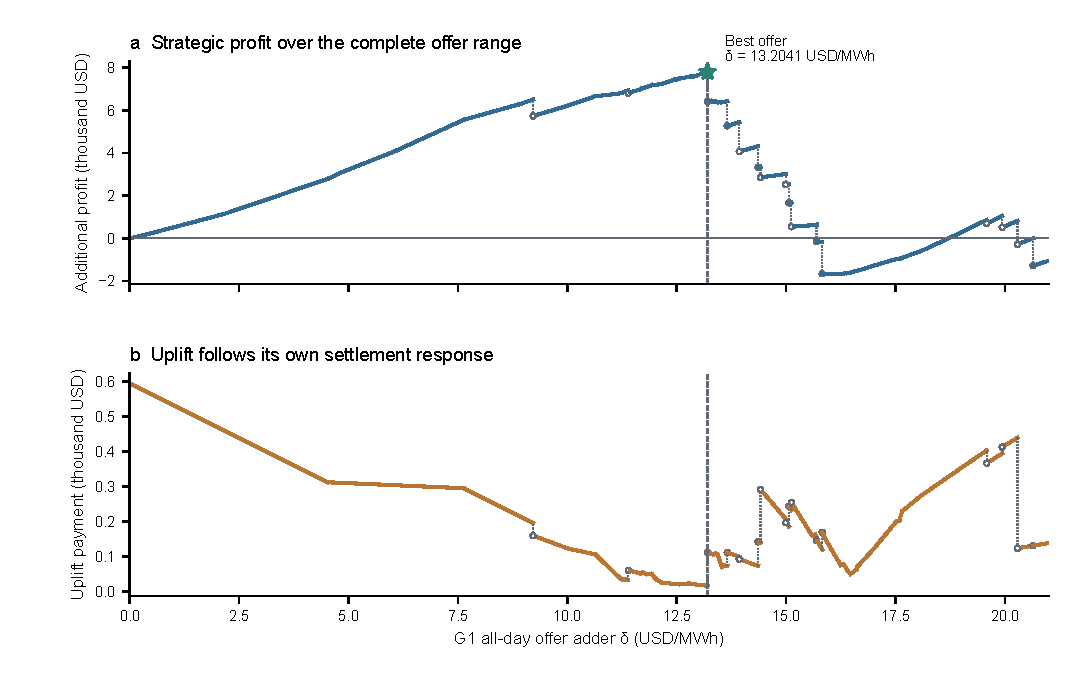
\includegraphics[width=\textwidth]{../paper_results/figures/fig3_strategic_profit_uplift.pdf}
\caption{G1 additional actual profit and uplift payment over the complete offer domain. Continuous pieces use common optimal physical and self-schedules. Dotted vertical indicators and open markers distinguish adjacent limits at physical switches; they do not interpolate attainable intermediate payoffs. The star denotes the declared higher-profit boundary candidate.}
\label{fig:profits}
\end{figure*}
\begin{table}[t]
\centering\caption{Settlement Changes at G1's Best Offer (USD)}\label{tab:settlement}
\setlength{\tabcolsep}{3.2pt}
\begin{tabular}{@{}lrrrr@{}}\toprule
Unit & $\Delta R_g$ & $\Delta U_g$ & $\Delta C_g$ & $\Delta\Pi_g$\\\midrule
G1&4385.61&$-578.36$&$-4004.31$&7811.56\\
G2&202.68&$-0.10$&252.45&$-49.87$\\
G3&$-5592.77$&$-508.42$&$-6742.11$&640.92\\
G4&0.00&0.00&0.00&0.00\\
G5&11707.21&$-312.43$&11394.79&0.00\\
G6&13.64&$-13.64$&0.00&0.00\\\bottomrule
\end{tabular}
\vspace{2pt}\parbox{\columnwidth}{\footnotesize Best offer minus truthful bidding under the same higher-profit boundary schedule. Each row satisfies $\Delta\Pi_g=\Delta R_g+\Delta U_g-\Delta C_g$. Other units keep their offers fixed.}
\end{table}
Figure~\ref{fig:profits} evaluates the entire G1 offer range. Actual profit increases from $37{,}289.31$ at truthful bidding to $45{,}100.87$ at $\delta^*=13.2040804436$ USD/MWh, an increment of $7{,}811.56$ or 20.95\% of baseline profit. The normalized offer adder is 31.4518\%. At the same candidate, uplift falls from $594.61$ to $16.26$. The opportunity to earn additional profit therefore persists while compensation declines.

Table~\ref{tab:settlement} explains the accounting. G1 energy revenue increases by $4{,}385.61$, uplift decreases by $578.36$, and actual cost decreases by $4{,}004.31$. Their combination produces the observed profit increment. Across the full path, the alternative mechanism decomposition is
\begin{equation}
 \Delta\Pi_{G1}=8741.60-29.23-900.82=7811.56.\label{eq:path-result}
\end{equation}
The terms are the price effect, the integrated offer-exposure effect, and two physical switching effects. Common self-schedules certify all 99 joint intervals for the plotted curves. The reconstruction agrees with all 116 original candidate records and with independently settled historical samples.

Other units experience different combinations of revenue and cost changes. G3 earns $640.92$ more despite lower energy revenue because its actual cost falls further. G5 earns $11{,}707.21$ more energy revenue but its higher actual cost and reduced uplift nearly exactly offset that increase. These are settlement responses to G1's strategy, not separate strategic profits for the other units. At system level, total uplift falls from $2{,}814.52$ to $1{,}401.57$. The transmission adjustment in~\eqref{eq:tx} falls from $548.26$ to $334.55$, and~\eqref{eq:network-settlement} holds with residuals below $1.5\times10^{-10}$ dollars.

\begin{figure*}[t]
\centering
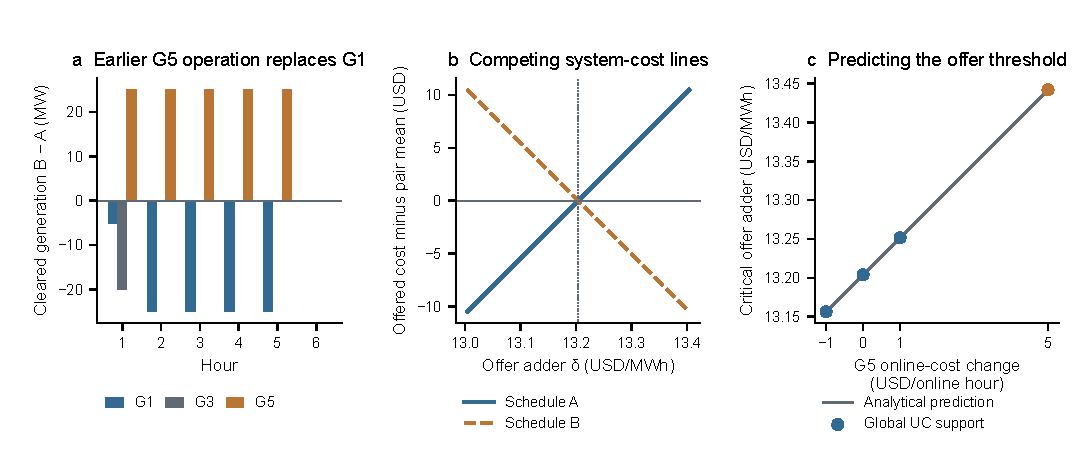
\includegraphics[width=\textwidth]{../paper_results/figures/fig4_substitution_threshold.pdf}
\caption{Physical substitution and the critical offer. (a) Cleared generation changes from schedule A to B in the first six hours. (b) Competing offered system-cost lines after subtracting their common offer-dependent pair mean, which preserves their crossing. (c) Predicted thresholds under specified changes in G5's actual online cost, supported by global UC checks.}
\label{fig:substitution}
\end{figure*}
An existing hour-specific comparison isolates the role of strategy timing. Raising only G1's hour-1 incremental offer over the same normalized 0--50\% range has a maximum additional profit of zero under its declared selector and physical-region rule. Two common physical regions and four endpoint/plan candidates support this conclusion. At the largest adder, actual profit is $37{,}182.90$, approximately $106.42$ below baseline, while uplift rises to $732.67$. Thus the same unit and market support a profitable all-day direction and a nonprofitable hour-1 direction. The admissible timing of offer changes is part of the market-power opportunity.

\subsection{Physical and Network Drivers of Market Power}

The critical offer reflects the cost of replacing G1 generation. In schedule A, G5 first operates in hour 6; in schedule B, it operates from hour 1. The additional five online hours provide 125 MWh and replace 105.069565 MWh from G1 and the remainder from G3. Both schedules start G5 once. Their actual system costs are $184{,}189.786589$ and $185{,}577.133581$, and their G1 offer-exposed quantities are 1464.060870 and 1358.991304 MWh. Equation~\eqref{eq:threshold} therefore predicts
\begin{equation}
 \delta^*=\frac{1387.346991}{105.069565}=13.204080444\ \mathrm{USD/MWh}.\label{eq:threshold-numeric}
\end{equation}
At this offer and the same selected CHP,~\eqref{eq:tie-profit} predicts a $1{,}387.35$ actual-profit difference between the two physical executions. The raw-precision settlement confirms it. A nearby offer $\delta^*-0.001$ still earns $7{,}810.84$ additional profit, so the profitable opportunity is also present immediately before the tie.

Figure~\ref{fig:substitution}(c) tests the cost mechanism. Increasing G5's actual online cost by $\epsilon$ dollars per online hour gives
\begin{equation}
 \delta^*(\epsilon)=13.204080444+0.047587519656\epsilon.\label{eq:prediction}
\end{equation}
The predefined $\epsilon=-1,0,1,5$ cases yield thresholds 13.15649, 13.20408, 13.25167, and 13.44202 USD/MWh. Global UC bounds at each crossing and neighboring offers support the candidate schedules. Increasing actual startup cost by \$50 per start leaves the threshold unchanged, as predicted by equal startup counts. These comparisons identify extra online operation as the relevant substitution expense in this transition.

The line-30 intervention then separates price effects from feasible competition. At the fixed offer $\delta^*-0.001$, relaxing line 30 lowers the hour-19 energy component from 114.8846 to 104.2192 USD/MWh. G5's congestion component rises from $-58.5446$ to $-45.9592$, so its nodal CHP increases from 56.34 to 58.26 despite the lower energy component. G5's cleared hour-19 output increases from 41.42 to 73.01 MW. The line-30 pricing multiplier becomes zero, while another line restriction remains active.

The relaxed system can also use a substitute schedule with a line-30 flow magnitude of approximately 39.01 MW, exceeding the original 20.8 MW limit. The original A/B schedules remain feasible and retain their mutual cost intersection, but the new schedule dominates them by approximately $2{,}196.5$ near that intersection. Transmission expansion changes the set of economic competitors that constrain G1's offer.

Finally, use each network's own truthful baseline. G1 baseline profit is $37{,}289.31$ in the original network and $31{,}911.46$ after relaxation. At $\delta^*-0.001$, total profit falls from $45{,}100.15$ to $40{,}302.15$, while additional profit rises from $7{,}810.84$ to $8{,}390.69$. Immediately above the original threshold, the corresponding increments are $6{,}424.82$ and $8{,}392.45$. These fixed-offer comparisons show how the direction of a market-power change can differ from the direction of a total-profit change. They connect the transmission price mechanism with the physical alternatives that the market can execute.

\section{Conclusion}
This paper develops a parametric CHP framework that reuses complete optimality information for continuous strategic offer evaluation. Common primal witnesses and complete dual interpolation produce affine selected-price maps. Combined with common physical UC regions, these maps reduce profit evaluation along a specified offer direction to finitely many endpoint/physical-plan candidates. Measured query workloads demonstrate how the initial mapping investment is amortized through repeated pricing.

The economic characterization links actual profit to reported self-scheduling profit and physical offer exposure. It explains profit differences between tied physical executions, separates local price and exposure effects, and predicts a substitution threshold from actual system costs. The principal case earns additional profit while both its own uplift and total system uplift decline. The transmission intervention further shows that network constraints shape nodal prices and the feasibility of generation replacement. Together, these results connect price vulnerability to profitable market power through explicit scheduling and settlement mechanisms.

\section*{Data and Code Availability}
The result tables, plotting data, implementation, numerical verification records, and supplementary self-scheduling witnesses are available in the \href{https://github.com/soda831143/CHP_pricing}{CHP\_pricing project repository}, under \path{chp_marketpower/paper_results}. The accompanying manuscript record identifies the source versions and the independent query workloads.

\section*{Acknowledgment}
OpenAI Codex assisted with source-code implementation, result organization, mathematical exposition, and preparation of this draft, including the text of Sections I--VI and plotting scripts. Numerical figures were rendered from archived optimization data. This statement records the assistance used in preparing the draft.

\bibliographystyle{IEEEtran}
\bibliography{references}
\end{document}
